\section{MapReduce}

MapReduce was introduced by Google in an attempt to to index massive volumes of data from a growing internet. This was outlined in a paper paper published in 2004 \cite{mapreduce}, a year later Hadoop was created. MapReduce solves the problem of distributed processing.

There are 2 stages in MapReduce. The first is the map stage and the second is the reducer stage. To describe the map and reduce stages we can use a simple but common example of counting words of a file outlined in the resarch paper\cite{mapreduce}. Our file could be a petabyte in size, for a normal desktop computer to process this file would be infeasible. However MapReduce makes this easy.

\subsection{Map}

As previously mentioned, a file can be split across multiple data nodes. Each data node has a block of data of the file, say 128 MB for each block. This is where the magic happens. Each data node can count the words only for each block of the file it is storing. This means that we can break the problem down substantially. If we have a 100 node cluster we can parallel process each block in a very short time frame. Our results from this stage are then gathered together in key value pairs and sent to the reduce phase. Figure \ref{fig:map-phase} below outlines the process.

\begin{figure}[H]
  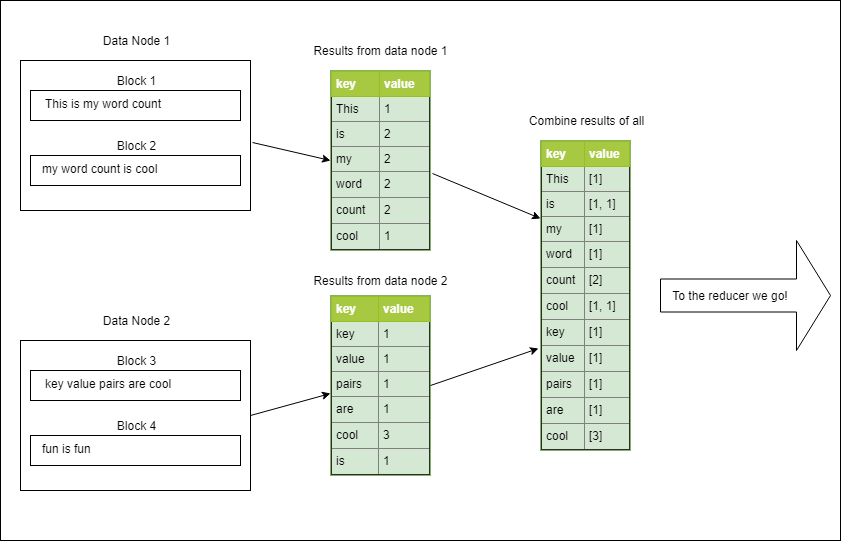
\includegraphics[width=\linewidth]{./images/map-phase.png}
  \caption{Map phase showing counting of words}
  \label{fig:map-phase}
\end{figure}

\subsection{Reduce}

The reduce phase takes the output of the map phase as its input. We then do some calculations on the data we have been presented with. In this case we are counting words. The value of each key from figure \ref{fig:map-phase} is a list of word counts, all we have to do is go through each key and sum up the values of the array. Next we return another key value pair with the completed word count and our MapReduce is complete. Figure \ref{fig:reduce-phase} outlines the reduce phase

\begin{figure}[H]
  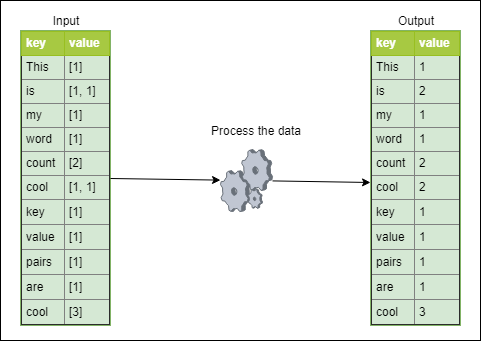
\includegraphics[width=\linewidth]{./images/reduce-phase.png}
  \caption{Reduce phase showing processing of word counts}
  \label{fig:reduce-phase}
\end{figure}

\subsection{How does this look in code?}

The creators of hadoop have done a great job abstracting away the underlying architecture. For example the coder does not have to to care that this will be running in parallel, possibly across hundreds of servers. Hadoop takes care of all this for us. 
Hadoop itself is mostly written in Java